% ============================================================
% CAPÍTULO 1 — A ARTE DE COMBINAR INFORMAÇÕES
% ============================================================

\chapter{A arte de combinar informações}

\begin{center}
\textit{Entre o que o modelo prevê e o que o instrumento observa, buscamos a melhor estimativa possível.}
\end{center}

\section*{Resumo}
Este capítulo apresenta a essência da \textbf{assimilação de dados} (AD): a arte e a ciência de combinar, de forma estatisticamente ótima, diferentes fontes de informação --- o modelo numérico e as observações --- para obter a melhor estimativa possível do estado real de um sistema físico, como a atmosfera.  
Partindo de uma visão intuitiva (interpolação ponderada) e evoluindo para a formulação estatística, introduz-se o conceito central de \textit{peso baseado em erro} e a transição entre o ``ajuste geométrico'' e a ``estimação probabilística''.

% ============================================================
\section{Entre o modelo e a realidade}
% ============================================================

A atmosfera é um sistema contínuo em espaço e tempo, mas nossas medições são \textbf{pontuais, esparsas e imperfeitas}.  
Em qualquer instante, conhecemos apenas uma fração do estado verdadeiro \( \mathbf{x}_t \).  
De acordo com \citet{Lorenc1986}, o problema da previsão numérica do tempo (PNT) é, essencialmente, um \textit{problema de condições iniciais}: pequenas incertezas no estado inicial podem amplificar-se exponencialmente devido à natureza caótica da atmosfera.  

\medskip
Para reduzir essa incerteza, introduz-se o conceito de \textbf{análise atmosférica} --- uma estimativa do estado tridimensional da atmosfera no instante de início da previsão.  
Essa análise deve incorporar tanto as observações disponíveis quanto o conhecimento prévio proveniente do modelo numérico.

\begin{tcolorbox}[colback=blue!3!white,title={Definição operacional de assimilação de dados}]
Segundo \citet{Kalnay2003}, \textit{assimilação de dados} é o processo de combinar, de forma coerente com as leis físicas e estatísticas, as \textbf{observações} e a \textbf{previsão de curto prazo do modelo} (ou \textbf{background}) para obter a melhor estimativa possível do estado do sistema}.
\end{tcolorbox}

Em notação moderna, o objetivo da assimilação é estimar o vetor de estado \( \mathbf{x}_a \in \mathbb{R}^n \) (análise) a partir de:
\begin{itemize}
  \item o \textbf{background} \( \mathbf{x}_b \), proveniente de uma previsão de curto prazo, normalmente de 6 ou 12 horas, gerada por um modelo de PNT;
  \item o vetor de \textbf{observações} \( \mathbf{y} \), obtido de instrumentos diversos (estações de superfície, sondagens, satélites, radares, boias etc.);
  \item o \textbf{operador de observação} \( \mathbf{H} \), que transforma as variáveis do modelo para o espaço de observação.
\end{itemize}

Assim, o problema da assimilação é formular matematicamente o melhor compromisso entre a \emph{consistência dinâmica do modelo} e a \emph{fidelidade das observações}.  
Em termos gerais:
\begin{equation}
\boxed{
\text{modelo (background)} + \text{observações} 
\;\longrightarrow\;
\text{análise (estado inicial ótimo)}.
}
\end{equation}

% ------------------------------------------------------------
\subsection*{Histórico e motivação}
% ------------------------------------------------------------

A necessidade de combinar dados observacionais e modelos preditivos surgiu nos anos 1950.  
\citet{Bergthorsson1955} propuseram o conceito de \textbf{``first guess''} --- uma estimativa inicial usada como ponto de partida para incorporar observações.  
Posteriormente, \citet{Gandin1963} formalizaram o problema de análise objetiva sob uma estrutura estatística, introduzindo o conceito de \textit{erro de background} e \textit{covariância espacial}.  

A evolução desse pensamento culminou com a formulação unificada de \citet{Lorenc1986}, que mostrou a equivalência entre os métodos de \textbf{Interpolação Ótima} (OI), \textbf{3DVar} e o \textbf{Filtro de Kalman}.  
Desde então, a assimilação de dados se consolidou como um campo que integra \textbf{física, estatística e ciência da computação}.

\begin{tcolorbox}[colback=gray!10!white,title={Comentário histórico}]
O avanço da assimilação de dados foi impulsionado por dois fatores principais:
\begin{enumerate}
  \item o aumento da densidade e diversidade das observações (principalmente por satélites);
  \item o crescimento do poder computacional, que tornou viável a solução iterativa de sistemas lineares e não lineares de alta dimensão.
\end{enumerate}
Hoje, centros globais como ECMWF, NCEP e JMA realizam análises globais a cada 6 horas, assimilando milhões de observações por ciclo.
\end{tcolorbox}

% ------------------------------------------------------------
\subsection*{Interpretação física}
% ------------------------------------------------------------

A assimilação pode ser vista como um processo de \textbf{fusão de informação física}:
\begin{itemize}
    \item O modelo numérico fornece coerência espaço-temporal e respeito às leis da dinâmica atmosférica, mas é afetado por simplificações e erros de parametrização;
    \item As observações trazem informação direta da realidade, mas são pontuais, ruidosas e distribuídas irregularmente.
\end{itemize}

A combinação desses dois mundos segue o princípio da \textbf{melhor estimativa estatística} --- formalizado por \citet{Kalman1960} e generalizado para sistemas atmosféricos por \citet{Lorenc1986}.  
Em termos conceituais, queremos encontrar o estado \( \mathbf{x}_a \) que minimize o erro médio quadrático esperado em relação ao estado verdadeiro \( \mathbf{x}_t \):

\begin{equation}
E\big[(\mathbf{x}_a - \mathbf{x}_t)(\mathbf{x}_a - \mathbf{x}_t)^{\mathrm{T}}\big] 
\;\; \text{mínimo.}
\end{equation}

Essa é a \textit{essência estatística} da assimilação de dados: um problema de estimação ótima sob incerteza.

% ------------------------------------------------------------
\subsection*{O ciclo de assimilação}
% ------------------------------------------------------------

Operacionalmente, a assimilação é realizada de forma cíclica (Figura~\ref{fig:cycle}), conforme descrito por \citet{Kalnay2003}:
\begin{enumerate}
    \item inicia-se com um campo de background \( \mathbf{x}_b \) obtido de uma previsão curta;
    \item são coletadas as observações válidas em uma janela de tempo centrada na análise;
    \item aplica-se o algoritmo de assimilação (OI, VAR, EnKF etc.) para obter a análise \( \mathbf{x}_a \);
    \item a análise é usada como condição inicial para o próximo ciclo de previsão, gerando um novo \( \mathbf{x}_b \).
\end{enumerate}

\begin{figure}[h!]
\centering
\begin{tikzpicture}[>=latex,line join=bevel]

  % ===================== PARÂMETROS GERAIS =====================
  \def\N{4}      % número de setas/etapas no anel
  \def\Gap{12}   % gap angular (graus) entre setas

  % Larguras angulares (calculadas para fechar 360° com N setas + N gaps)
  \pgfmathsetmacro{\Span}{(360-\N*\Gap)/\N} % largura de cada seta (graus)
  \pgfmathsetmacro{\Step}{\Span+\Gap}       % passo angular entre centros
  \pgfmathtruncatemacro{\Nm}{\N-1}          % inteiro seguro p/ foreach

  % Raios do anel (controle da “grossura” das setas)
  \def\Rin{3.05}
  \def\Rmid{3.45}
  \def\Rout{3.95}
  \def\Tip{7}    % “ponta” da seta em graus (3–8 costuma ficar bonito)

  % Fundo (anéis de referência e raio das caixas)
  \def\Cin{\Rin-1.05}     % círculo interno do halo
  \def\Cout{\Rout+0.15}   % raio base para posicionar as caixas

  % ================ FUNDO / HALO (opcional) ====================
  \fill[even odd rule,gray!10] circle (\Cout) circle (\Cin); % halo
  \fill[white,opacity=.90] circle (2.05);                    % miolo claro

  % ================ ESTILOS DE COR PARA AS SETAS ===============
  % Use arrow/0,...,arrow/3. Para mais etapas, defina arrow/4, arrow/5, etc.
  \tikzset{
    arrow/0/.style = {fill=teal!30,   draw=teal!70!black,  very thick, line width=1.2pt},
    arrow/1/.style = {fill=green!30,  draw=green!60!black, very thick, line width=1.2pt},
    arrow/2/.style = {fill=orange!40, draw=orange!70!black,very thick, line width=1.2pt},
    arrow/3/.style = {fill=blue!30,   draw=blue!70!black,  very thick, line width=1.2pt},
    % Estilo das caixas externas:
    infobox/.style = {
      draw=black!40, rounded corners=2.2mm, fill=white, drop shadow,
      text width=4.0cm, align=center, inner sep=4pt
    }
  }

  % ===================== DESENHO DAS ETAPAS =====================
  % Lista robusta com 4 campos: índice / ângulo / âncora / texto.
  % OBS: as âncoras devem ser válidas no TikZ: east, west, north, south.
  %      O ângulo (\theta) determina a direção radial da caixa.
  \foreach \i/\theta/\anch/\etapa in {
    0/  25/west/{\textbf{Previsão curta (modelo)}\\Gera $\mathbf{x}_b$ para a janela seguinte},
    1/ 120/south/{\textbf{Coleta \& CQ das observações}\\Janela centrada na análise; filtros e QC},
    2/ 215/east/{\textbf{Análise (assimilação)}\\$\mathbf{x}_a=\mathbf{x}_b+\mathbf{K}\bigl(\mathbf{y}-\mathcal{H}(\mathbf{x}_b)\bigr)$},
    3/ 305/north/{\textbf{Condições iniciais}\\Propaga $\mathbf{x}_a$ para o próximo ciclo}
  }{
    % Centro e limites angulares da seta i
    \pgfmathsetmacro{\center}{\i*\Step}
    \pgfmathsetmacro{\astart}{\center-0.5*\Span}
    \pgfmathsetmacro{\aend}{\center+0.5*\Span}

    % Seta (texto interno curto: “etapa i”; pode trocar por {} se não quiser texto)
    \arcarrow{\Rin}{\Rmid}{\Rout}{\astart}{\aend}{\Tip}{arrow/\i}{etapa \i}

    % Caixa da etapa i (posição polar: ângulo \theta, raio \Cout)
    %  - anchor=\anch prende a caixa pelo lado indicado (east/west/north/south)
    \node[infobox,anchor=\anch] at (\center:\Cout) {\etapa};
  }

  % ======================= TÍTULO CENTRAL =======================
  \node[align=center, text=black!75]
   {\bfseries Ciclo de \\ \bfseries Assimilação de Dados \\
    Integração contínua\\ modelo e observações\\
    (\textit{novo ciclo})};

\end{tikzpicture}


\caption{Esquema conceitual de um ciclo de assimilação de dados atmosféricos. Cada ciclo integra previsões curtas e novas observações para atualizar o estado do sistema.}
\label{fig:cycle}
\end{figure}

Esse processo iterativo é o núcleo de qualquer sistema moderno de previsão numérica, garantindo que a informação observacional seja continuamente incorporada no modelo.

% ------------------------------------------------------------
\subsection*{Síntese conceitual}
% ------------------------------------------------------------

\begin{tcolorbox}[colback=yellow!5!white,title={Síntese}]
A assimilação de dados:
\begin{itemize}
    \item reconhece explicitamente que tanto o modelo quanto as observações possuem erro;
    \item combina essas duas fontes de informação com base em suas \textbf{covariâncias de erro};
    \item produz uma estimativa estatisticamente ótima do estado atmosférico;
    \item mantém coerência temporal e física através do ciclo modelo--análise.
\end{itemize}
Em outras palavras, ela é o \textbf{elo entre a teoria, a observação e a modelagem numérica} --- um processo que transforma dados brutos em conhecimento preditivo sobre o Sistema Terrestre.
\end{tcolorbox}


% ============================================================
\section{Interpolação como estimativa ponderada}
% ============================================================

Antes de pensar em estatística, é útil lembrar que a ideia de \textbf{combinar informações} já existia implicitamente na \textbf{interpolação clássica}.  
Nela, a estimativa \( \hat{z}(x_0) \) em um ponto \( x_0 \) é uma média ponderada das observações conhecidas \( z(x_i) \):

\begin{equation}
\hat{z}(x_0) = \sum_{i=1}^{N} w_i(x_0)\, z(x_i),
\qquad 
\sum_{i=1}^{N} w_i(x_0) = 1.
\label{eq:interp}
\end{equation}

Os \textbf{pesos} \( w_i(x_0) \) dependem da distância entre o ponto de interesse e as observações.  
Um exemplo clássico é o \textbf{peso gaussiano}:

\begin{equation}
w_i(x_0)
= 
\dfrac{
\exp\!\left[-\dfrac{(x_0 - x_i)^2}{R^2}\right]
}{
\sum_{j=1}^{N} 
\exp\!\left[-\dfrac{(x_0 - x_j)^2}{R^2}\right]
},
\label{eq:gaussian_weight}
\end{equation}
onde \( R \) é o \textbf{raio de influência}.  
Quanto menor a distância \(|x_0 - x_i|\), maior o peso de \(z(x_i)\) na estimativa.

\medskip
\noindent
\textbf{Interpretação física.}  
A interpolação ponderada já é, implicitamente, uma filtragem espacial: as observações mais próximas (ou mais confiáveis) dominam a estimativa.  
Essa ideia inspirou a \textbf{análise objetiva} \citep{Cressman1959,Barnes1964} --- o elo direto com a assimilação moderna.

% ============================================================
\section{Transição para pesos baseados em erro}
% ============================================================

A grande revolução conceitual da assimilação moderna foi substituir o critério geométrico (distância) por um \textbf{critério estatístico (erro)}.  

Denotemos:
\begin{itemize}
    \item \( \mathbf{x}_b \) --- vetor de background (previsão de curto prazo);
    \item \( \mathbf{y} \) --- vetor de observações;
    \item \( \mathbf{H} \) --- operador que mapeia o estado do modelo para o espaço de observação;
    \item \( \mathbf{K} \) --- matriz de ganho (ou de ponderação ótima).
\end{itemize}

A análise é dada por:
\begin{equation}
\boxed{
\mathbf{x}_a = \mathbf{x}_b + \mathbf{K}\,(\mathbf{y} - \mathbf{H}\mathbf{x}_b)
}
\label{eq:analysis}
\end{equation}
em que o termo \(\mathbf{d} = \mathbf{y} - \mathbf{H}\mathbf{x}_b\) é a \textbf{inovação} (diferença observação--background).

A matriz \(\mathbf{K}\) define o peso ótimo de cada informação:
\begin{equation}
\boxed{
\mathbf{K} = \mathbf{B}\,\mathbf{H}^\mathrm{T}\,
(\mathbf{H}\mathbf{B}\mathbf{H}^\mathrm{T} + \mathbf{R})^{-1}},
\label{eq:kalman_gain}
\end{equation}
onde  
\(\mathbf{B}\) é a covariância de erro de background e  
\(\mathbf{R}\) é a covariância de erro de observação.

Essas matrizes determinam quanto se confia no modelo ou nas observações:

\begin{center}
\begin{tabular}{|c|c|}
\hline
Situação & Consequência \\
\hline
\( \mathbf{B} \gg \mathbf{R} \) & observações recebem maior peso \\
\( \mathbf{R} \gg \mathbf{B} \) & o modelo prevalece \\
\( \mathbf{B} \sim \mathbf{R} \) & combinação equilibrada \\
\hline
\end{tabular}
\end{center}

\noindent
\textbf{Interpretação.}  
A AD é uma \textit{interpolação ponderada por incertezas}, ou seja, uma fusão estatisticamente fundamentada entre modelo e dados.

% ============================================================
\section{Exemplo escalar --- o caso BLUE 1D}
% ============================================================

Considere uma variável escalar \(z\) observada (\(z_o\)) e prevista pelo modelo (\(z_b\)).  
Suponha erros não correlacionados, com variâncias \(\sigma_o^2\) e \(\sigma_b^2\).  
A melhor estimativa linear não enviesada (BLUE, \textit{Best Linear Unbiased Estimator}) é:
\begin{equation}
z_a = 
\dfrac{z_b/\sigma_b^2 + z_o/\sigma_o^2}
      {1/\sigma_b^2 + 1/\sigma_o^2}.
\label{eq:blue}
\end{equation}

ou, de modo equivalente,
\begin{equation}
z_a =
w_b\,z_b + w_o\,z_o,
\qquad
w_b = \dfrac{1/\sigma_b^2}{1/\sigma_b^2 + 1/\sigma_o^2},
\quad
w_o = \dfrac{1/\sigma_o^2}{1/\sigma_b^2 + 1/\sigma_o^2}.
\end{equation}

Se o modelo erra mais (\(\sigma_b^2\) grande), \(w_o\) domina; se as observações são mais ruidosas (\(\sigma_o^2\) grande), \(w_b\) domina.  
A Eq.~\eqref{eq:blue} é a forma unidimensional das Eqs.~\eqref{eq:analysis} e~\eqref{eq:kalman_gain}.

% ------------------------------------------------------------
\begin{tcolorbox}[title={Ligação com mínimos quadrados},colback=gray!5!white]
Minimizar o erro médio quadrático entre a análise e o estado verdadeiro \(x_t\) leva exatamente à Eq.~\eqref{eq:kalman_gain}.  
A matriz \(\mathbf{K}\) surge como solução do problema:
\[
\min_{\mathbf{K}} 
E\big[(\mathbf{x}_a - \mathbf{x}_t)(\mathbf{x}_a - \mathbf{x}_t)^\mathrm{T}\big].
\]
Derivando e anulando o gradiente, obtém-se a solução de Kalman.  
Portanto, o ganho de Kalman é o \textbf{operador de mínimos quadrados generalizado}.
\end{tcolorbox}

% ============================================================
\section{Representação visual (pgfplots)}
% ============================================================

\begin{figure}[h!]
\centering
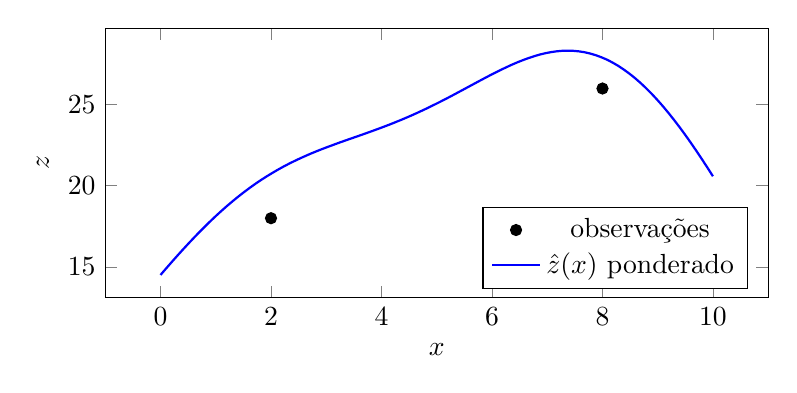
\begin{tikzpicture}
\begin{axis}[xlabel={$x$}, ylabel={$z$}, width=10cm, height=5cm, legend pos=south east]
\addplot[only marks, mark=*] coordinates {(2,18) (8,26)};
\addlegendentry{observações};
\addplot[domain=0:10,samples=100,blue,thick]{18*exp(-(x-2)^2/16)+26*exp(-(x-8)^2/16)};
\addlegendentry{$\hat{z}(x)$ ponderado};
\end{axis}
\end{tikzpicture}
\caption{Interpolação 1D entre duas observações usando pesos gaussianos normalizados (raio efetivo \(R\approx4\)).}
\label{fig:interp1d}
\end{figure}

\begin{figure}[h!]
\centering
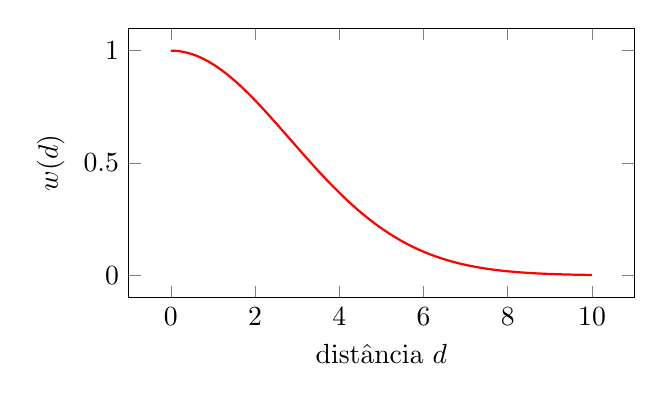
\begin{tikzpicture}
\begin{axis}[xlabel={distância $d$}, ylabel={$w(d)$}, width=8cm, height=5cm]
\addplot[domain=0:10,samples=100,red,thick]{exp(-x^2/16)};
\end{axis}
\end{tikzpicture}
\caption{Função de peso gaussiana típica utilizada em análises espaciais: o peso decai rapidamente com a distância em relação ao raio \(R\).}
\label{fig:gaussian}
\end{figure}

% ============================================================
\section{Interpretação física e probabilística}
% ============================================================

Sob a ótica probabilística,  
\begin{itemize}
    \item o background é uma amostra da distribuição \( \mathcal{N}(\mathbf{x}_t, \mathbf{B}) \);
    \item as observações, uma amostra de \( \mathcal{N}(\mathbf{H}\mathbf{x}_t, \mathbf{R}) \).
\end{itemize}
A análise é a média ponderada dessas duas distribuições --- o ponto em que o \textbf{produto das probabilidades} é máximo.  
Ou seja, o vetor \( \mathbf{x}_a \) é o \textbf{valor de máxima verossimilhança} sob hipóteses gaussianas.

% ============================================================
\section{Síntese}
% ============================================================

A interpolação fornece a intuição básica: estimar valores nos vazios, combinando vizinhança e suavidade.  
A assimilação de dados amplia esse conceito ao incluir \textbf{incertezas estatísticas} e formular a estimativa como uma \textbf{combinação ótima} de modelo e observação.

\begin{equation}
\text{Interpolação} 
\;\Rightarrow\;
\text{Mínimos Quadrados} 
\;\Rightarrow\;
\text{Análise Objetiva} 
\;\Rightarrow\;
\text{Assimilação Estatística (VAR, EnKF, Kalman)}.
\end{equation}

Nos capítulos seguintes, formalizaremos essa transição passo a passo --- do ajuste por mínimos quadrados à formulação completa da assimilação moderna.

% ============================================================
\section*{Referências}
% ============================================================

\begin{thebibliography}{99}
\bibitem[Cressman(1959)]{Cressman1959} Cressman, G. P. (1959). \textit{An operational objective analysis system}. Mon. Wea. Rev., 87, 367--374.
\bibitem[Barnes(1964)]{Barnes1964} Barnes, S. L. (1964). \textit{A technique for maximizing detail in numerical weather map analysis}. J. Appl. Meteor., 3, 396--409.
\bibitem[Kalnay(2003)]{Kalnay2003} Kalnay, E. (2003). \textit{Atmospheric Modeling, Data Assimilation and Predictability}. Cambridge Univ. Press.
\bibitem[Lorenc(1986)]{Lorenc1986} Lorenc, A. C. (1986). \textit{Analysis methods for numerical weather prediction}. Q. J. R. Meteorol. Soc., 112, 1177--1194.
\bibitem[Evensen(2009)]{Evensen2009} Evensen, G. (2009). \textit{Data Assimilation: The Ensemble Kalman Filter}. Springer.
\end{thebibliography}
